\section{Experimental setup}\label{sec:setup}

\paragraph{Arms and cells.}
The pipeline runs twice, producing two arms that differ in exactly one thing: the input text.
The \textbf{raw} arm uses the opening document as the source system holds it; the
\textbf{anonymised} arm uses the same document after the suppression step of
Section~\ref{sec:anon}. Everything else --- feature blocks, parameters, seeds, evaluation
protocol --- is identical, which is what makes the difference between arms attributable to
anonymisation rather than to some other choice.

Each arm yields \textbf{seven} clusterings: three algorithm families in a reference
configuration plus four parameter variants --- a coarser density variant that merges clusters
below a distance threshold, two centroid variants with $k$ chosen by the elbow criterion and by
the silhouette respectively, and one modularity variant at a different resolution. That is
\textbf{fourteen} real clusterings, each paired with its own shuffled control
(Section~\ref{sec:controls}), hence \textbf{twenty-eight} partitions. Every partition is
evaluated on the \textbf{three} trace alphabets of Section~\ref{sec:alphabets}, giving
\textbf{84} evaluation cells. Within a cell, six generator families are fitted per cluster above
the 30-trace floor: a third-order Markov chain, GRU, LSTM and Transformer, a graph-convolutional
model, and a directly-follows graph which under top-1 prediction coincides with the
within-cluster successor baseline. Across the 84 cells this comes to 4{,}323 cluster evaluations
and \textbf{25{,}938} fitted generators. Figure~\ref{fig:pipeline} summarises the stages.

\begin{figure}[htbp]
\centering
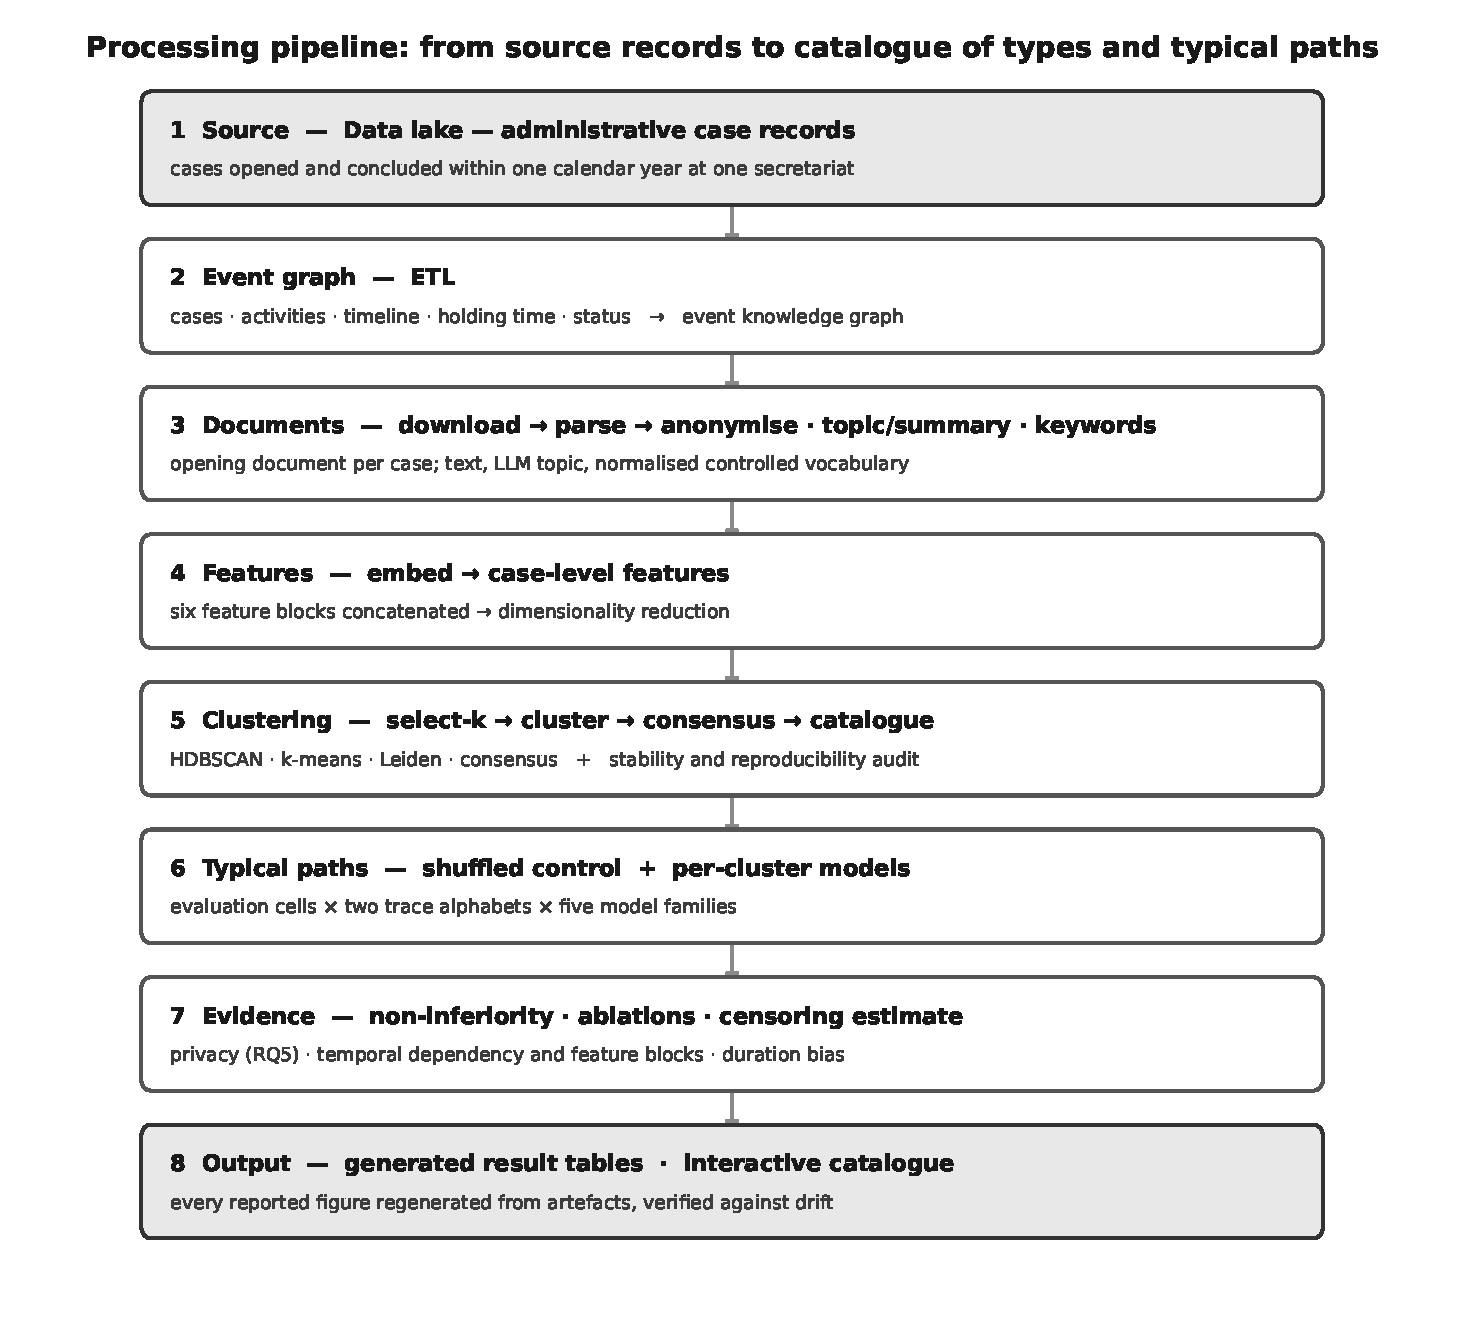
\includegraphics[width=0.86\textwidth]{pipeline-macro-en.pdf}
\caption{Pipeline from source event log to catalogue and generated evidence tables.}
\label{fig:pipeline}
\end{figure}

\paragraph{Controls.}
The shuffled-partition control is generated by permuting the labels of a real clustering, which
preserves cluster count, size distribution and the population that survives the evaluation
floor, so the only difference from the real partition is membership. The list of control cells
is derived from the list of real cells by the stage that runs them, rather than written
alongside it, so the two cannot diverge without failing.

\paragraph{The evidence layer.}
The stages above produce the artefact; the ones that follow exist to try to knock it down, and
each answers an objection a sceptical reader would be right to raise. All of them run per
alphabet wherever the quantity they measure depends on the alphabet.

\begin{itemize}
  \item \textbf{Block and history ablation} --- \emph{is it the documentary content that groups,
    or would anything group?} Feature blocks are zeroed one at a time and each case's history is
    truncated, measuring how far the partition moves.
  \item \textbf{Corpus bias} --- \emph{do the cases that conclude within the year represent the
    cases opened in it?} Right-censoring is estimated month by month (Section~\ref{sec:bias})
    rather than assumed benign.
  \item \textbf{Temporal holdout} --- \emph{does the advantage survive when the partition sees
    only part of each case's history?} The cuts are rescored over the cases all of them evaluate,
    since otherwise different populations would be compared.
  \item \textbf{Non-inferiority} --- \emph{does suppressing personal data cost utility, against a
    margin fixed before measuring?}
  \item \textbf{Constraint cost} --- \emph{what does the validity guarantee charge the
    generator?}
  \item \textbf{Conformance} --- \emph{how much of the observed behaviour does the discovered
    model reproduce, and how much more does it permit?}
  \item \textbf{Stability} --- \emph{does the partition survive resampling of its own members?}
  \item \textbf{Refit audit} --- \emph{does each stored clustering reproduce from the feature
    matrix it declares?}
  \item \textbf{Control partition} --- introduced in Section~\ref{sec:controls} and formalised in
    Section~\ref{sec:estimand}, the one that decides whether any of the others has anything to
    act on.
\end{itemize}

One lesson, methodological before it is empirical, organises the whole layer: \textbf{the
comparator decides the answer}. The same models, over the same cases, support different claims
according to what they are measured against --- which is why this study fixes its estimand before
measuring and reports the comparator beside every number.

\paragraph{Choosing among admitted partitions.}
$\Delta^{*}$ decides which partitions enter the study but does not order them
(Section~\ref{sec:estimand}). To choose among the admitted ones we use an explicit score with
three terms and weights declared in advance: \textbf{downstream performance}, weight 0.5,
measured over the \emph{common set} --- the cases that \emph{every} partition evaluates, without
which performance would be compared over different populations --- and scaled from the floor the
best shuffled partition reaches; \textbf{coverage}, weight 0.3, the fraction of the corpus that
survives the 30-trace floor; and \textbf{internal quality}, weight 0.2, the mean of two rescaled
validity indices. The weights are a choice, so the decision is put through a sensitivity sweep
over five weighting schemes --- balanced, downstream-first, coverage-first, quality-first and
equal thirds --- reporting the winner under each. A choice that survives only one weighting is a
choice of the weighting.

\paragraph{Reproducibility.}
Feature matrices are stamped with a digest of their inputs, and the clustering and evaluation
stages refuse to run against features whose stamp does not match the arm they claim --- a guard
rather than a convention. An audit stage refits each stored clustering from its own stamped
matrix, replays the recipe that clustering declares, including the noise policy of
Section~\ref{sec:noise}, and compares the result to the stored labels; its outcome is reported in
Section~\ref{sec:res-rq1}. A second audit walks the whole artefact tree and checks that every
file still declares the stage that produced it and that the declared inputs still digest the same
way. That chain --- question, version, inputs, refit --- is what turns ``this was run'' into
``anyone can re-run this''.

Document and topic embeddings are cached on disk, so switching arms restores identical vectors
rather than recomputing them; we verified that a raw--anonymised--raw cycle leaves the feature
matrix unchanged. A document whose anonymised text is byte-identical to its raw text keeps the
vector it already has rather than being reprocessed. It is not excluded, but it contributes no
anonymisation signal either, and the stage records how many documents are in that condition.

\paragraph{From artefacts to this paper.}
Every quantitative table in this paper is generated from stored artefacts by a single pipeline
stage, which also regenerates the corresponding tables in the project's internal results
document. A verification mode re-renders both the manuscript's tables and the internal
document's and fails if either has drifted from the artefacts, so a figure cannot be edited into
a table without the underlying evidence changing first. The complete grid of parameter
combinations is not printed here; it is regenerable from the stored artefacts.

Generated tables are the easy half. The numbers a reader actually encounters are in prose, and
prose is hand-written; a regeneration check cannot see it. We therefore maintain a second check,
run with the test suite, that holds an explicit register of the load-bearing quantitative claims
in the running text, resolves each to its path in the artefact tree, and fails in either
direction --- if a figure in the prose no longer rounds to the artefact it cites, or if the
artefact changes and the sentence is not updated with it. The register includes sign assertions,
so a rewording that preserves a magnitude while erasing the sign of a result also fails. It is
not exhaustive, and we make the narrower claim it supports: the figures it covers cannot drift
silently, and any figure not in it is verified only by reading.

\paragraph{Statistical procedures.}
The comparison between the raw and anonymised arms uses a paired bootstrap over the cases both
arms evaluate, with 2{,}000 replicates, conducted per alphabet and never across alphabets. The
pair is the case rather than the cell, which removes from the interval the variation due to case
difficulty. A conclusion of non-inferiority requires the one-sided 90\% lower bound of the
difference to clear a margin of 0.01 accuracy points, registered before the data existed, and a
sensitivity margin of 0.005 is reported alongside so that the conclusion's robustness to the
choice of margin is visible rather than assumed.

The relationship between a partition's internal quality and its downstream quality is tested by
rank correlation under a Monte Carlo permutation test with 20{,}000 draws, over the fourteen real
parameterisations of a single alphabet. Eight quantities are tested: four internal validity
indices --- DBCV, silhouette, Davies--Bouldin and Calinski--Harabasz --- and four descriptors of
partition shape --- cluster count, median cluster size, final noise rate, and the fraction density
would refuse before the assignment of Section~\ref{sec:noise}. All are tested without correction
for multiplicity, and all require the indices to come from one \emph{metric space}: indices
computed in different spaces are not comparable and cannot be pooled into a single correlation, so
the procedure aborts rather than silently aggregate a partition from outside the common space.

That design has low power, and the power is a property of the design rather than of the outcome:
with fourteen observations at $\alpha = 0.05$ the test rejects only for $|\rho| \geq 0.534$, and
attains 80\% power only near $|\rho| = 0.75$. The statement rule is therefore fixed before the
result is known: absent rejection we report absence of evidence and make no equivalence claim
about the indices, because the procedure alone establishes neither.
